% !TEX root=../main.tex

\section{Examples}
\label{sec:examples}

This section introduces three example \TOPHAT programs.
Each example illustrate different functionality of the \TOPHAT language.
\cref{sec:vending} demonstrates the step combinator, \cref{sec:tax} includes the parallel and choice combinators, and finally \cref{sec:dining} demonstrates the use of shares in order for tasks to communicate with each other.
The examples will be used in \cref{sec:assistive} to demonstrate how \ASTOPHAT works, and are included in the implementation described in \cref{sec:implementation}.


\subsection{Vending Machine}
\label{sec:vending}

Using the editors and combinators described in \cref{sec:tophat},
we can create a vending machine that dispenses a biscuit for one coin and a chocolate bar for two coins as follows:


\begin{TASK}[
    float=ht,
    numbers=right,
    caption={Vending machine dispensing biscuits or chocolate.},
    captionpos=b,
    label=lst:vending]
  let vend : Task Snack = edit 0 >>? \n. $\label{lst:vend:enter}$
    if n == 1 then edit Biscuit             $\label{lst:vend:branch}$
    else if n == 2 then edit ChocolateBar
    else fail                               $\label{lst:vend:fail}$
\end{TASK}

This example demonstrates the usage of a user step guarded by a branching expression (\cref{lst:vend:branch}) using the failure task (\cref{lst:vend:fail}).
The editor $\Edit 0$ asks the user to enter an amount of money.
It simulates a coin slot in a real machine that freely accepts and returns coins.
There is a continue button, generated by the user step combinator $\Next$.
Only when the user has inserted exactly 1 or 2 coins will the continue button become enabled.
Other cases will result in the failure task $\Fail$, and stepping to it is prohibited by definition.
When the user presses the continue button, the machine dispenses either a biscuit or a chocolate bar, depending on the amount of money.
Snacks are modelled using a custom type.


\subsection{Tax subsidy request}
\label{sec:tax}

The example program listed in this section is taken from our previous work on symbolic execution for \TOPHAT~\cite{DBLP:conf/ppdp/SteenvoordenNK19}.
It models a simplified tax subsidy application process for citizens who have installed solar panels.
This was first described by Stutterheim~et~al.\cite{conf/sfp/StutterheimAP17},
who worked on modelling a fictional but realistic law about solar panel subsidies.

A subsidy is only given under the following conditions.
\begin{itemize}
\item The roofing company has confirmed that they installed solar panels for the citizen.
\item The tax officer has approved the request.
\item The tax officer can only approve the request if the roofing company has confirmed, and the request is filed within one year of the invoice date.
\item The amount of the granted subsidy is at most €600.
\end{itemize}

\lstset{emph={invoiceDate,confirmed,invoiceAmount,approved}}
\begin{TASK}[
    float=ht,
    numbers=right,
    caption={Subsidy request and approval workflow at the Dutch tax office.},
    captionpos=b,
    label=lst:tax]
  let today = $\Today$ in
  let provideDocuments = enter Amount <&> enter Date in
  let companyConfirm = edit True <?> edit False in
  let officerApprove = \ invoiceDate. \ today. \ confirmed.
    edit False <?> if (today - invoiceDate < $\OneYear$ /\ confirmed) $\label{lst:tax:officer-approve-def}$ then edit True else fail in
  provideDocuments <&> companyConfirm >>= \ <<<<invoiceAmount, invoiceDate>>, confirmed>>. $\label{lst:tax:documents-and-company-confirm}$
  officerApprove invoiceDate today confirmed >>= \ approved.$\label{lst:tax:officer-approve}$
  let subsidyAmount = if approved then min 600 (invoiceAmount / 10) else 0 in
  edit <<subsidyAmount, approved, confirmed, invoiceDate, today>>$\label{lst:tax:result}$
\end{TASK}

\Cref{lst:tax} gives the \TOPHAT code for this example.
To enhance readability of the example,
we omit type annotations and make use of pattern matching on tuples.
The program works as follows.

In parallel, the citizen has to provide the invoice documents of the installed solar panels, while the roofing company has to confirm that they have actually installed solar panels at the citizen's address (\cref{lst:tax:documents-and-company-confirm}).
Once the invoice and the confirmation are there, the tax officer has to approve the request (\cref{lst:tax:officer-approve}).
The officer can always decline the request, but they can only approve it if the roofing company has confirmed and the application date is within one year of the invoice date (\cref{lst:tax:officer-approve-def}).
The result of the program is the amount of the subsidy, together with all information needed to prove the required properties (\cref{lst:tax:result}).

In previous work, we have shown that this code indeed adheres to the requirements listed above.
There we focussed on assisting the developer by proving the program correct.
In this work we focus on supporting the end user that is requesting a subsidy.
The end user wants the outcome of this program to be a subsidy amount larger than zero.
In \cref{sec:assistivetax} we will show how to generate hints for the end user to reach this goal.


\subsection{Dining Computer Scientists Problem}
\label{sec:dining}

The dining philosophers problem is a classic concurrency problem in computer science.
A number of philosophers sit at a round table with a meal in front of them.
In between the plates lies a fork.
In order to eat their meal, each philosopher has to acquire two forks.
Only after eating his or her meal, is a philosopher allowed to place the two forks back on the table.
This, of course, means that the philosophers cannot eat at the same time, since there are not enough forks.
Deadlock can occur when all philosophers pick up the fork to their right (or left).
Then, everybody has one fork.
This means that each philosopher cannot start his or her meal, and is also not allowed to put his fork back on the table.\\

\noindent
\begin{minipage}[r]{0.55\textwidth}

\lstset{emph={this, that, name, left, right}}
\begin{TASK}[
    %float=ht,
    numbers=right,
    caption={Dining philosophers problem with three computer scientists.},
    captionpos=b,
    label=lst:dining]
  let fork0 = ref True in $\label{lst:phil:fork0}$
  let fork1 = ref True in $\label{lst:phil:fork1}$
  let fork2 = ref True in $\label{lst:phil:fork2}$
  let pickup = \ this. \ that. $\label{lst:phil:this}$
    if !this $\label{lst:phil:deref}$
      then edit this := False >>? \ _. $\label{lst:phil:mark-used}$
        if !that then edit this := True else fail $\label{lst:phil:that}$
      else fail in
  let scientist = \ name. \ left. \ right. $\label{lst:phil:scientist}$
    pickup left right <?> pickup right left in $\label{lst:phil:pick}$
  scientist "Alan Turing" fork0 fork1 <&> $\label{lst:phil:scientist0}$
  scientist "Grace Hopper" fork1 fork2 <&> $\label{lst:phil:scientist1}$
  scientist "Ada Lovelace" fork2 fork0 >>= \ _ . $\label{lst:phil:scientist2}$
    edit "Full bellies"
\end{TASK}
\end{minipage}
\begin{minipage}[r]{0.05\textwidth}
  \
\end{minipage}
\begin{minipage}[r]{0.4\textwidth}
\tikzset{every picture/.style={line width=0.75pt}} %set default line width to 0.75pt

  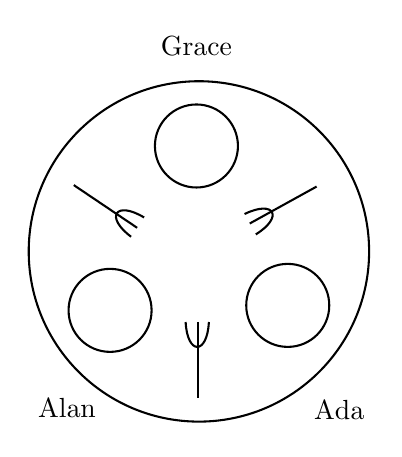
\begin{tikzpicture}[x=0.75pt,y=0.75pt,yscale=-0.8,xscale=0.8]
  %uncomment if require: \path (0,300); %set diagram left start at 0, and has height of 300

  %Shape: Circle [id:dp8519268538531043]
  \draw   (229,147.5) .. controls (229,90.89) and (274.89,45) .. (331.5,45) .. controls (388.11,45) and (434,90.89) .. (434,147.5) .. controls (434,204.11) and (388.11,250) .. (331.5,250) .. controls (274.89,250) and (229,204.11) .. (229,147.5) -- cycle ;
  %Shape: Circle [id:dp8204933417548707]
  \draw   (305,84) .. controls (305,70.19) and (316.19,59) .. (330,59) .. controls (343.81,59) and (355,70.19) .. (355,84) .. controls (355,97.81) and (343.81,109) .. (330,109) .. controls (316.19,109) and (305,97.81) .. (305,84) -- cycle ;
  %Shape: Circle [id:dp7478076126793654]
  \draw   (360,180) .. controls (360,166.19) and (371.19,155) .. (385,155) .. controls (398.81,155) and (410,166.19) .. (410,180) .. controls (410,193.81) and (398.81,205) .. (385,205) .. controls (371.19,205) and (360,193.81) .. (360,180) -- cycle ;
  %Shape: Circle [id:dp3120260710082954]
  \draw   (253,183) .. controls (253,169.19) and (264.19,158) .. (278,158) .. controls (291.81,158) and (303,169.19) .. (303,183) .. controls (303,196.81) and (291.81,208) .. (278,208) .. controls (264.19,208) and (253,196.81) .. (253,183) -- cycle ;
  %Straight Lines [id:da6820891014633774]
  \draw    (331,190) -- (331,236) ;


  %Curve Lines [id:da1548185264621137]
  \draw    (323.5,190) .. controls (324.5,210) and (336.5,210) .. (337.5,190) ;



  %Straight Lines [id:da4306446303925887]
  \draw    (294.3,133.27) -- (256.15,107.56) ;


  %Curve Lines [id:da9253738091345234]
  \draw    (298.49,127.05) .. controls (281.34,116.7) and (274.64,126.65) .. (290.66,138.66) ;



  %Straight Lines [id:da7927760692654279]
  \draw    (362.12,130.68) -- (402.39,108.44) ;


  %Curve Lines [id:da6105283277592903]
  \draw    (365.75,137.25) .. controls (382.77,126.7) and (376.97,116.2) .. (358.98,124.99) ;




  % Text Node
  \draw (252,242) node  [align=left] {Alan};
  % Text Node
  \draw (330,24) node  [align=left] {Grace};
  % Text Node
  \draw (416,243) node  [align=left] {Ada};


  \end{tikzpicture}
  \vspace{0.7cm}
  \captionof{figure}{Rendering with three philosophers.}
\end{minipage}\\
\\
We look at dining computer scientists instead.
\cref{lst:dining} lists an implementation in \TOPHAT for this problem, with three computer scientists.
The forks are represented by references containing Booleans (\cref{lst:phil:fork0,lst:phil:fork1,lst:phil:fork2}).
Using references allows tasks to communicate with each other without passing values on directly.
Reading a reference $l$ is denoted as $!l$, assigning a new value $v$ to a reference $l$ is written as $l:=v$.
The value $\True$ indicates that the fork is available,
$\False$ indicates that the fork is being used.

Picking up a fork is only possible when the fork is available,
i.e reading the reference results in $\True$ (\cref{lst:phil:deref}).
This fork is then marked as being used (\cref{lst:phil:mark-used}).
The use of references ensures that the neighbouring scientist cannot pick up this fork: this choice will be disabled.
After that, one can press continue if the second fork is also available (\cref{lst:phil:that}).
For the sake of simplicity, one returns the first fork, rather than setting the second fork to $\False$, and then setting both to $\True$ again.

Each computer scientist takes as arguments a name and references to the two forks that he or she can reach (\cref{lst:phil:scientist}).
They have a choice to take either the left or the right fork.
This is represented with an user choice ($\Xor$, \cref{lst:phil:pick}).
The last lines instantiate three computer scientists sitting next to each other (\cref{lst:phil:scientist0,lst:phil:scientist1,lst:phil:scientist2}).
In \TOP terms, this means they collaborate in parallel ($\And$) while eating their dinner, sharing some resources,
in this case $\lbl{fork0}$, $\lbl{fork1}$, and $\lbl{fork2}$.

By design of \TOPHAT, the events of picking up a fork are performed sequentially.
That is, when one computer scientist decides to pick up his right fork, we will handle that event first.
After that, we will handle the choices from the other scientists.
So, the order of the events is explicitly determined by the scientists themselves.
% This is regardless of choices interfering or not.

In \cref{sec:assistivedining} we will analyse this example.
Our goal is to provide each scientist with a hint on which choice to make, in order to reach the common goal of full bellies.
When the scientists follow these hints, no deadlock will occur.
